\section{Работа с программной моделью \MyProc}
\label{ch::asm}


Программная модель позволяет создавать и отлаживать программы для \MyProc. По желанию пользователя может быть установлен русский или английский язык пользовательского интерфейса.

\subsection{Главное окно приложения}

Вид главного окна приложения представлен на рисунке \ref{fig:asm:r8asmWindow}. Пользователь при желании может сменить язык интерфейса на английский, выбрав пункт меню <<Справка / Язык интерфейса / English>> и перезапустив приложение.

В строке статуса приложения (нижняя часть главного окна) пользователь может выбрать свой набор команд. Рекомендуется реализовать алгоритм в нулевом наборе, выполнить отладку и тестирование, а затем выполнить переход в свой, ограниченный набор команд.

\begin{figure}
    \centering
    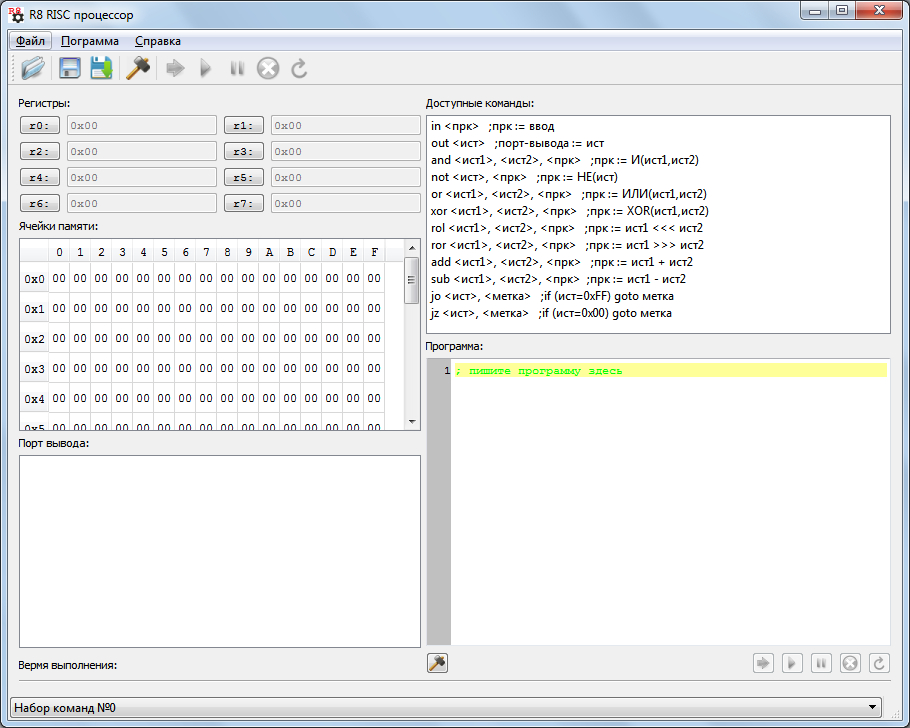
\includegraphics[width=\textwidth]{fig/r8asmWindow}
    \caption{Главное окно программной модели {\MyProc} (русский язык интерфейса)}\label{fig:asm:r8asmWindow}
\end{figure}

В главном окне программной модели отображается:
\begin{itemize}
    \item Номер текущнего набора команд RISC-процессора \MyProc.
    
    \item Состояние всех восьми регистров процессора \MyProc. Щелчок на имени регистра приводит к последовательному переключению отображения значения регистра в одну из систем счисления: двоичную, восьмеричную, шестнадцатеричную, десятичную.
    
    \item Состояние всех ячеек памяти процессора \MyProc. Значение в ячейке памяти изображается в шестнадцатеричной системе счисления.
    
    \item История вывода в порт вывода. Отображается выведенное значение в шестнадцатеричной, двоичной и десятичной системах счисления.
    
    \item Условное время выполнения программы в тактах. Правила подсчета времени выполнения приведены в разделе \ref{ch:risc:time}.
    
    \item Над областью редактора кода отображается список команд для выбранного набора с кратким описанием логики их работы.
    
    \item Область редактора позволяет в любой момент редактировать программу, отображает точки останова, а также отмечает текущую команду в режиме пошаговой отладки. Редактирование программы в процессе её отладки завершает отладку автоматически.
    
    \item Под областью редактора располагаются кнопки для выполнения основных команд отладки программы. Подробности отладки приводятся в разделе \ref{ch:asm:debug}
\end{itemize}


\subsection{Работа с редактором кода}

Редактор кода предназначен для комфортной работы с исходным текстом \MyProc-программы на языке ассемблера. Реализована подсветка синтаксиса (рисунок \ref{fig:asm:syntaxhighlight}), что облегчает редактирование программы и позволяет избежать большинства ошибок компиляции. В разном стиле подсвечиваются константы, мнемоники команд, регистры, комментарии и метки. Синтаксические ошибки подчеркиваются красной волнистой линией.

\begin{figure}
    \centering
    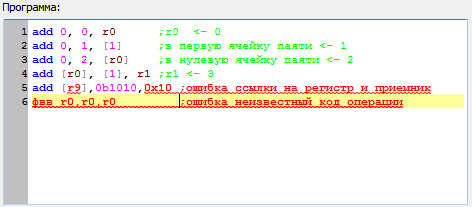
\includegraphics{fig/syntaxhighlight}
    \caption{Редактор {\MyProc} с подсветкой синтаксиса и ошибок}\label{fig:asm:syntaxhighlight}
\end{figure}

Пример отладки программы определения переноса (см. теорию в разделе \ref{ch:risc:p}) приведен на рисунке \ref{fig:asm:r8asmEditor}.

\begin{figure}
    \centering
    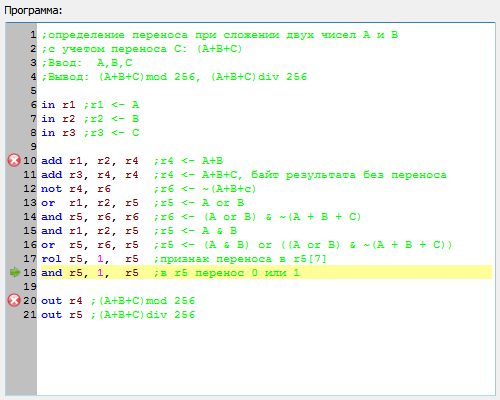
\includegraphics{fig/r8asmEditor}
    \caption{Редактор {\MyProc} в процессе отладки}\label{fig:asm:r8asmEditor}
\end{figure}

% ;определение переноса при сложении двух чисел A и B
% ;с учетом переноса С: (A+B+C)
% ;Ввод: A,B,C
% ;Вывод: (A+B+C)mod 256, (A+B+C)div 256
% ;r6 --- для промежуточных результатов
% in r1 ;r1 <- A
% in r2 ;r2 <- B
% in r3 ;r3 <- C 
%  
% add r1, r2, r4  ;r4 <- A+B
% add r3, r4, r4  ;r4 <- A+B+C, байт результата без переноса
% not r4, r6      ;r6 <- ~(A+B+c)
% or  r1, r2, r5  ;r5 <- A or B
% and r5, r6, r6  ;r6 <- (A or B) & ~(A + B + C)
% and r1, r2, r5  ;r5 <- A & B
% or  r5, r6, r5  ;r5 <- (A & B) or ((A or B) & ~(A + B))
% rol r5, 1,  r5  ;признак переноса в r5[7]
% and r5, 1,  r5  ;в r5 перенос 0 или 1
% 
% out r4 ;(A+B+C)mod 256
% out r5 ;(A+B+C)div 256

Исходный текст программы на языке ассемблера {\MyProc} можно сохранить в файл, используя соответствующие команды главного меню или кнопки на панели быстрого доступа: <<Файл / Сохранить>> или <<Файл / Сохранить как\ldots>>. Точки останова при этом не сохраняются.

Исходный текст также может быть загружен с помощью команды <<Файл / Открыть>>.


\subsection{Компиляция и отладка программы}
\label{ch:asm:debug}

Для отладки программы на языке ассемблера {\MyProc} можно выполнить следующие команды:
\begin{itemize}
    \item Перевести в машинный код (
\includegraphics[width=16pt]{fig/r8asm/image/compile}). Выполнить трансляцию мнемоник команд ассемблера {\MyProc} в машинный код {\MyProc}. Когда компиляция проходит без ошибок, становятся доступными команды отладки. Ошибки компиляции выводятся в окно порта вывода и строка, в которой обнаружена ошибка, подсвечивается.
    
    \item Выполнить команду (
\includegraphics[width=16pt]{fig/r8asm/image/step}). Пошаговый режим выполненя команд: выполняется текущая команда и выполняется останов на следующей. Текущая команда отмечается в редакторе соответствующим значком. После выполнения команды отображается новое состояние процессора.
    
    \item Выполнить программу (
\includegraphics[width=16pt]{fig/r8asm/image/run}). Выполнятеся программа целиком или выполняется переход в пошаговый режим на точке останова (
\includegraphics[width=16pt]{fig/r8asm/image/breakpoint}). 
    
    \item Останов (
\includegraphics[width=16pt]{fig/r8asm/image/stop}). Выполнятеся останов на текущей команде и переход в пошаговый режим.
    
    \item Точка останова (
\includegraphics[width=16pt]{fig/r8asm/image/breakpoint}). Выполнятеся установка точки останова в текущей строке редактора. Это не влияет на режим выполнения команд. При редактировании исходного текста, точки останова остаются в тех позициях, в которых были установлены.
    
    \item Перезапуск (
\includegraphics[width=16pt]{fig/r8asm/image/restart}). Выполнятеся сброс процессора и переход в пошаговый режим выполнения программы, начиная с первой команды.    
\end{itemize}
